\documentclass{article}

\usepackage[margin=1in]{geometry}
\usepackage[T1]{fontenc}
\usepackage[fontsize=11pt]{fontsize}
\usepackage{fancyhdr}
\usepackage{extramarks}
\usepackage{amsmath}
\usepackage{amsthm}
\usepackage{amsfonts}
\usepackage{tikz}
\usepackage[plain]{algorithm}
\usepackage{algpseudocode}
\usepackage{multicol}
\usepackage{hyperref}

\usetikzlibrary{automata,positioning}

\linespread{1}

\pagestyle{fancy}
\lhead{\hmwkAuthorName}
\chead{\hmwkClass: \ \paprTitle}
\rhead{\today}
\lfoot{\hmwkTitle}
\cfoot{\thepage}

\renewcommand\headrulewidth{0.25pt}
\renewcommand\footrulewidth{0.25pt}

\setlength\columnseprule{.25pt}
\setlength{\columnsep}{2.5pc}
\setcounter{secnumdepth}{0}


\newcommand{\hmwkTitle}{Assignment\ \#3}
\newcommand{\paprTitle}{\\ A Report on Infor EAP}
\newcommand{\hmwkDueDate}{May 31, 2023 @ 23:59, EST}
\newcommand{\hmwkClass}{CIS 562 - Enterprise Architecture}
\newcommand{\hmwkAuthorName}{\textbf{Cason Konzer}}


\title{
    \vspace{2in}
    \textmd{\textbf{\hmwkClass:\ \\ \hmwkTitle}}\\
    \normalsize\vspace{0.1in}\small{Due\ on\ \hmwkDueDate}\\
    \vspace{0.1in}\Large{\textit{\paprTitle}}
    \vspace{3in}
}

\author{\hmwkAuthorName}
\date{\today}

\begin{document}

\maketitle

\pagebreak

\tableofcontents
\listoftables
\listoffigures
\newpage


\section{Introduction}
In this report we will be discussing Infor, a multinational software company. 
In specific focus is Infor's ERP (Enterprise Resource Planning) offerings, EAP (Enterprise Application Platform), and factors driving their market demand. 
With many large competing firms such as Oracle, Microsoft, and SAP, these factors are crucial to why or why not an enterprise will choose Infor as the preferred ERP supplier. 

\subsection{History}

Founded in 2002, Infor started as Agilisys, before growing into the company we know today through a plethora of acquisitions.
Notably: In 2004 Infor acquired ERP company Infor Business Solutions (additionally renaming Agilisys to Infor Global Solutions), in 2006 ERP company SSA Global, in 2011 ERP company Lawson Software, and in 2017 BI (Business Intelligence) company Birst.
The company has remained privately owned throughout it life, initially backed by Golden Gate Capital and now Koch Equity Development LLC \cite{wikipedia_infor}. 

The core of today's ERP offerings from Infor can be traced back to their 2011 ION (Intelligent Open Network) offering. 
Still early in their venture, Infor adopted a platformed approach, hereafter referred to as EAP, of which ION represents.
As an EAP, ION brought Infor and third-party ERP products into a centralized location, enabling business to seamlessly integrate workflows across services and easily onboard new softwares. 

Initially EAPs were offered as a hosted (on-premise) platform, seen now most frequently as PaaS (Platform as a Service) offerings. 
In 2014 Infor started ERP integrations into the cloud on AWS (Amazon Web Services), becoming the first ERP vendor to provide cloud based offerings.
It was not long before ION API Gateway was offered to bridge cloud ERP systems with hosted systems.
In a similar manner, by 2017 Infor had joined multiple offerings into Infor OS (Operating Services), and released their EAP as a PaaS cloud consumable \cite{infor_os_next_gen}.

In the recent years Infor has released new offerings such as AI (Artificial Intelligence) and ML (Machine Learning) for digital assistants, document management, and process intelligence. 
Appealing to market demand, no/low-code dashboards have been incorporated for application development to drive a satisfactory UX (User Experience).
It is through Infor's EAP that traditional ERP system offerings are integrated such as: Finance and accounting, supply chain management, planning and scheduling, project, customer and order management \cite{infor_erp, infor_eai_ml_os}. 
Current today, Infor's ERP solutions are a small fraction of their EAP (Figure~\ref{fig:Infor_EAP}), driving business value though integration with third-party ERP solutions via their Data Extract (ETL).

\section{Market Factors}
In order to evaluate Infor in the ERP market we will focus on a cloud ERP implementation detailed in \cite{critical_cloud_erp}. 
In comparing Infor to other suppliers we leverage their product-market fit given distinct use cases and capabilities given below.

\begin{multicols}{2}
\begin{itemize}
    \item[] \textbf{Use Cases}
    \item[$\diamond$] ERP for Midsize Enterprises
    \item[$\diamond$] ERP for Large and Global Enterprises
    \item[$\diamond$] Discrete Manufacturing
    \item[$\diamond$] Project/Asset-Intensive Manufacturing
    \item[$\diamond$] Process Manufacturing
    \item[$\diamond$] Distribution of Goods
\end{itemize}

\begin{itemize}
    \item[] \textbf{Capabilities}
    \item[$\ast$] Single-Vendor ERP Suite Solution
    \item[$\ast$] Complex Corporate Requirements
    \item[$\ast$] Geographic Coverage
    \item[$\ast$] Discrete Manufacturing
    \item[$\ast$] Complex Manufacturing
    \item[$\ast$] Process Manufacturing
    \item[$\ast$] Distribution, Warehouse, Logistics
    \item[$\ast$] Support/SI/Methodology
    \item[$\ast$] Advanced Technology
    \item[$\ast$] Composable Platform
    \item[$\ast$] Financial Management
\end{itemize}
\end{multicols}

Capabilities are assigned weights to each use case and defined in Table~\ref{tab:cap_by_use}.
Vendor ratings are calculated by their capabilities and then aggregated to determine their use case market fit. 
Detailed capability ratings are provided, although for brevity we will report only those most critical to Infor. 

\subsection{Benefits}

Generally speaking, Infor is well rounded and one of the top cloud ERP suppliers for all use cases, classified as an industry leader by the authors of \cite{critical_cloud_erp} in \cite{magic_cloud_erp}.
Their top use cases fall under ERP for midsize enterprises, discrete manufacturing, and process manufacturing (Figure~\ref{fig:Infor_Benefits}).

Across all vendors, Infor was rated as the most capable of providing a single-vendor ERP suite solution, scoring a 4.7/5. 
The attribution of this rating depends critically on their long term research and development in EAP. 
As a result this benefit drives Infor's dominance in ERP for midsize enterprises, while buffing their discrete manufacturing domain expertise. 
In a similar manner, Infor was rated highest in process manufacturing, critical to the process manufacturing use case, and a slight factor in in ERP for midsize enterprises.
Yet again, Infor set the state of the art in discrete manufacturing capabilities.

Distribution, warehouse, logistics carry the highest average weight and factor into every use case, of which Infor ranked second, giving them a good all-around buff. 
Of the remaining capabilities which were not a direct challenge to Infor, they tied for second in composable platform, and third in advanced technology.

\subsection{Challenges}
Continuing on to Infor's challenges, a clear distinguishing factor is their tie for last place in support/SI/methodology. 
This capability drove weakness especially so in ERP for large and global enterprises, project/asset-intensive manufacturing, and distribution of goods, their worst scoring use cases (Figure~\ref{fig:Infor_Challenges}).

In financial management, Infor ranked fourth, diminishing their application to ERP for large and global enterprises.
Similarly, Infor was fourth in complex corporate requirements and complex manufacturing, driving key downgrades in ERP for large and global enterprises and project/asset-intensive manufacturing respectively. 

\section{Conclusion}
In conclusion, enterprises have many reasons in which Infor may be viewed as the provider of choice. 
Granted, some recommendation to the team may help them outpace even the largest of publicly traded leaders. 
Building upon the cautions mentioned in \cite{magic_cloud_erp}, my suggestion to Infor is to build up additional technical support, expand their partnership arrangements with third-party software providers, and increase flexibility and transparency in their licensing practices. 
In summary, improving customer relations through support/SI/methodology capabilities would play the most influential role in their ratings. 

\newpage

\section{Appendix : Tables}

\begin{table}[h!]
    \centering
    \begin{tabular}{|c||c|c|c|c|c|c|} 
        \hline
        \          & Midsize & Large \& Global & Discrete & Proj./Asset & Process & Dist. \\
        \hline
        \hline
        Single-Vendor Suite     &  41 \%  &  0  \%  &  8  \%  &  3  \%  &  0  \%  &  10 \% \\
        \hline
        Complex Requirements    &  0  \%  &  20 \%  &  5  \%  &  4  \%  &  1  \%  &  3  \% \\
        \hline
        Geographic Coverage     &  3  \%  &  25 \%  &  5  \%  &  4  \%  &  2  \%  &  10 \% \\
        \hline
        Discrete Manufacturing  &  10 \%  &  4  \%  &  45 \%  &  8  \%  &  0  \%  &  0  \% \\
        \hline
        Complex Manufacturing   &  2  \%  &  10 \%  &  10 \%  &  45 \%  &  5  \%  &  0  \% \\
        \hline
        Process Manufacturing   &  5  \%  &  5  \%  &  0  \%  &  0  \%  &  62 \%  &  0  \% \\
        \hline
        Dist., Warehouse, Log.  &  8  \%  &  5  \%  &  10 \%  &  12 \%  &  10 \%  &  56 \% \\
        \hline
        Support/SI/Methodology  &  8  \%  &  10 \%  &  5  \%  &  10 \%  &  5  \%  &  8  \% \\
        \hline
        Advanced Technology     &  16 \%  &  8  \%  &  9  \%  &  5  \%  &  10 \%  &  10 \% \\
        \hline
        Composable Platform     &  3  \%  &  6  \%  &  3  \%  &  6  \%  &  5  \%  &  3  \% \\
        \hline
        Financial Management    &  4  \%  &  7  \%  &  0  \%  &  3  \%  &  0  \%  &  0  \% \\
        \hline
    \end{tabular}
    \caption{Capability Weights by Use Case \cite{critical_cloud_erp}.}
    \label{tab:cap_by_use}
\end{table}

\newpage

\section{Appendix : Figures}

\begin{figure}[ht!]
    \centering
    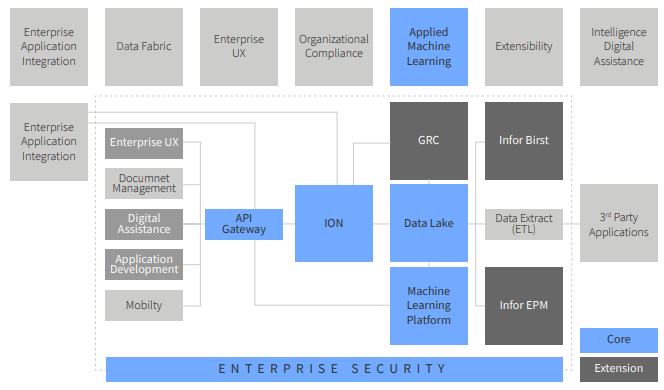
\includegraphics[width=\textwidth]{./Infor_EAP.PNG}
    \caption{Simplified architecture for applied machine learning with Infor OS \cite{infor_eai_ml_os}.}
    \label{fig:Infor_EAP}
\end{figure}

\newpage

\begin{figure}[ht!]
    \centering
    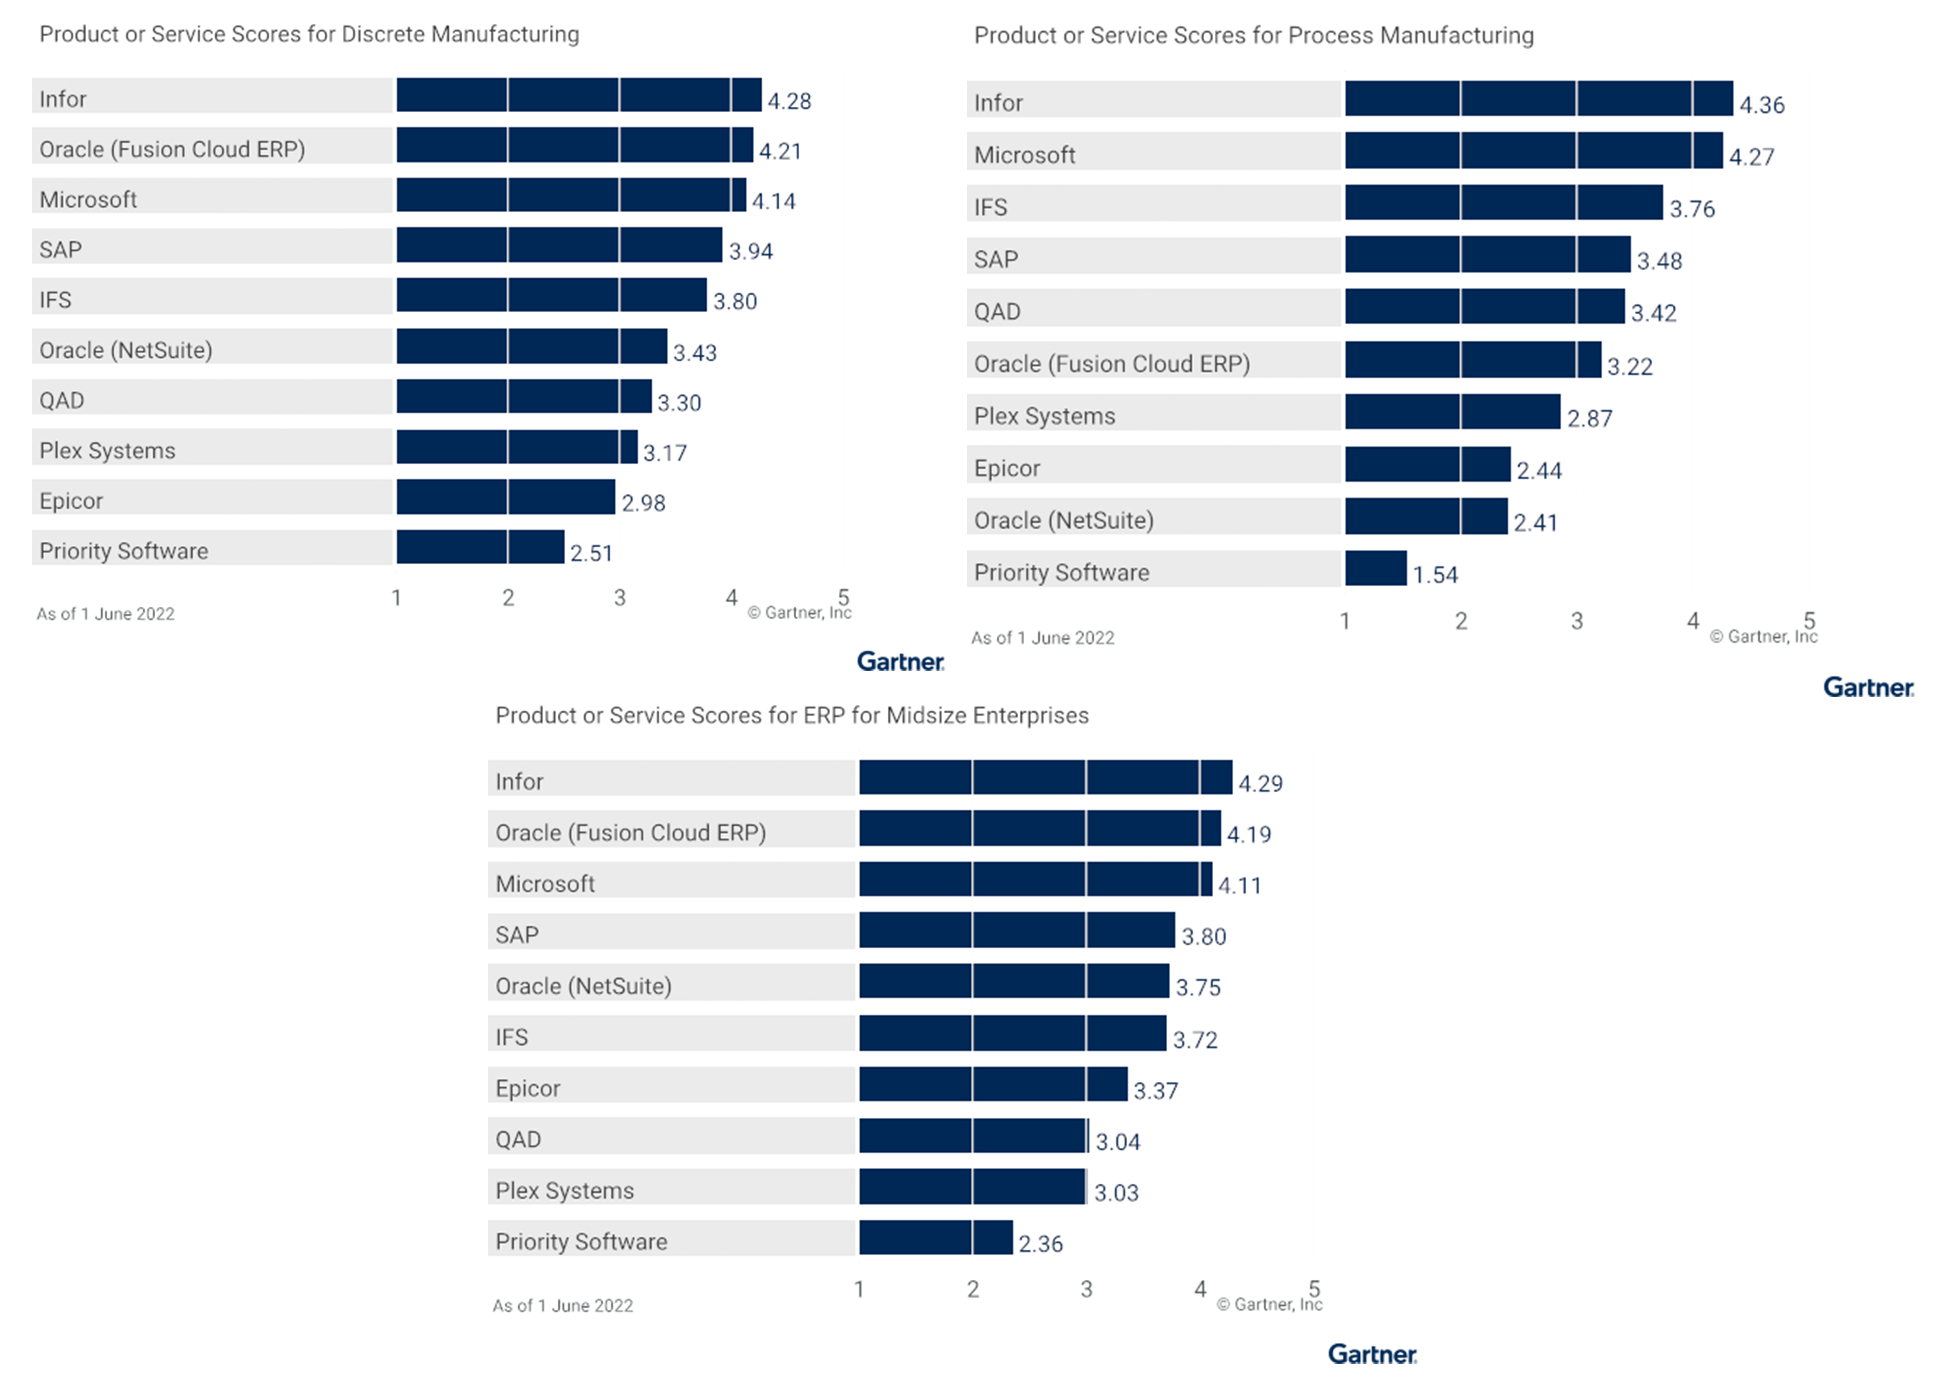
\includegraphics[width=\textwidth]{./Infor_Benefits.png}
    \caption{Infor Cloud ERP Use Case Benefits \cite{critical_cloud_erp}.}
    \label{fig:Infor_Benefits}
\end{figure}

\newpage

\begin{figure}[ht!]
    \centering
    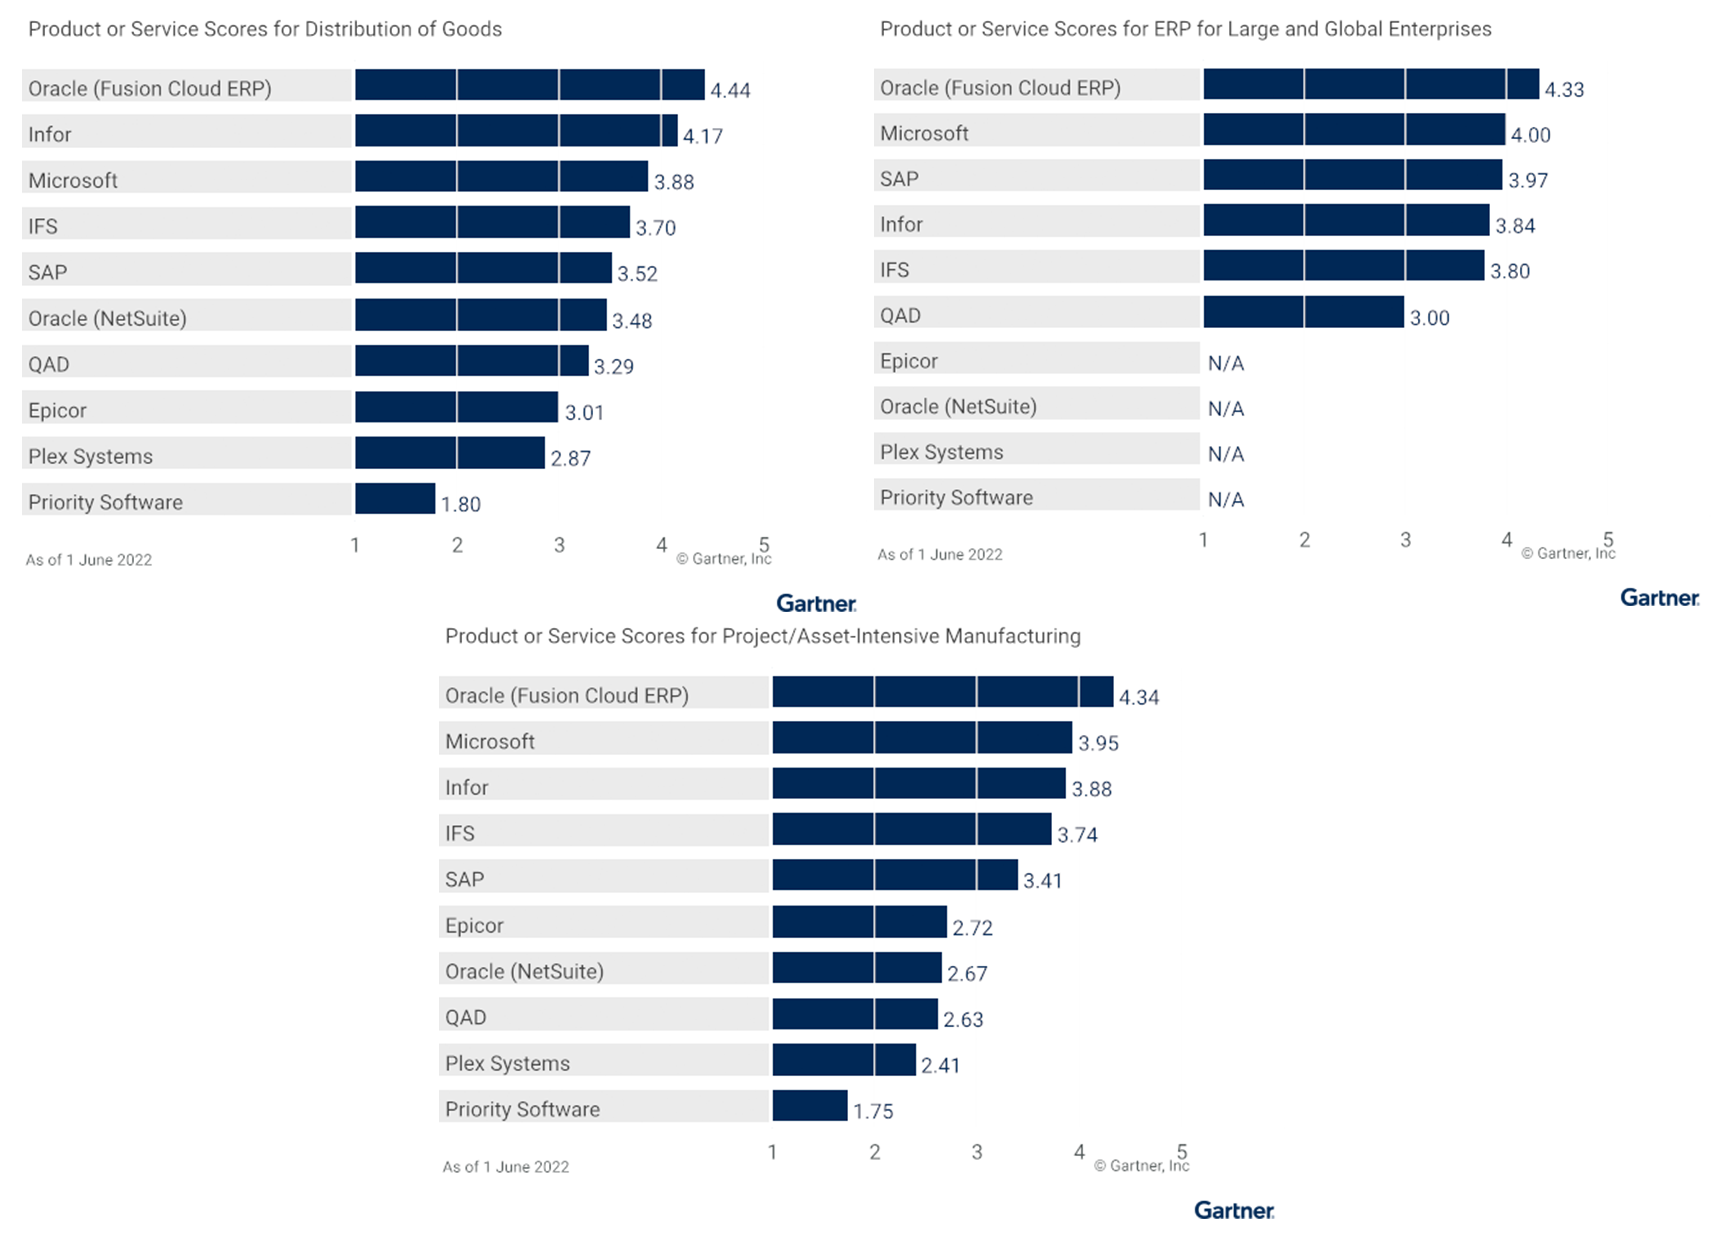
\includegraphics[width=\textwidth]{./Infor_Challenges.png}
    \caption{Infor Cloud ERP Use Case Challenges \cite{critical_cloud_erp}.}
    \label{fig:Infor_Challenges}
\end{figure}

\newpage

\bibliography{./konzer_cason_CIS_562_assignment_3.bib}{}
\bibliographystyle{naturemag} % abbrv, acm, alpha, apalike, ieeetr, plain, siam, unsrt, tugboat, perception, munich, naturemag
\end{document}